\section{System Architecture}
\hspace{2cm}To achieve its goal, our project is divided into several main modules which are integrated together in an appropriate manner, these modules are as follows:\\
\begin{enumerate}
    \item Web server
    \item Path planning
    \item Neural network 
    \item Main controller
    \item Convolutional Neural Network
    \item Classical control
    \item Obstacle avoidance
    \item Localization 
\end{enumerate}
These modules work on data from IMU, GPS, LIDAR and Webcam then send actions to Arduino to perform the tasks required by the client. An overview of the architecture is shown below in figure \ref{fig:system_arch}

  \begin{figure}[H]%
    \center%
    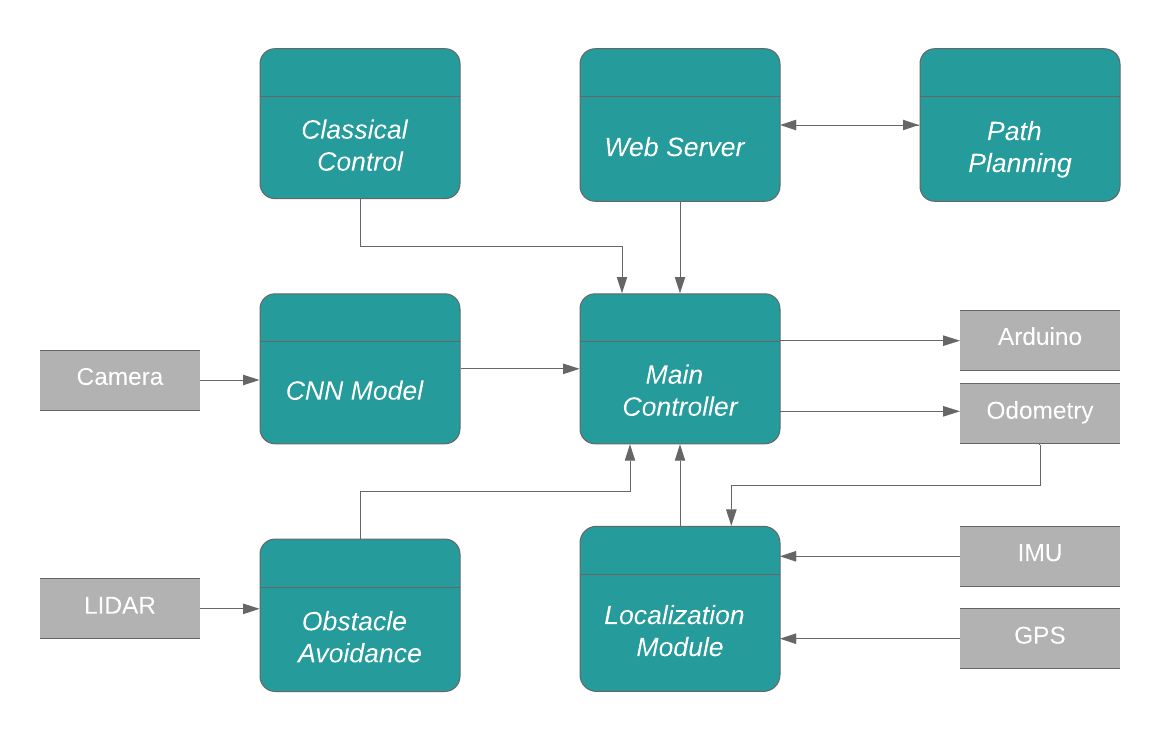
\includegraphics[width=\textwidth]
    {images/Alzahraa/system_arch.png}%
     % you need to add the caption for the list of figures
    \caption[System Architecture]{System Architecture}\label{fig:system_arch}%
  \end{figure}
  
\subsection{Web Server}
\hspace{2cm}The Web Service process resides on the web server. After the customer’s order is processed by the backend on the web server, An HTTP POST request is made to web server on the main device containing the task data.

\subsection{Path Planning}
\hspace{2cm}The path planning module takes the source and destination locations and generates the best path between them as several continuous nodes, then it sends the path to the main controller through the web server.

\subsection{Main Controller}
 \hspace{2cm}The main controller takes in all the control actions from CNN, classical control, obstacle avoidance modules and based on the current information provided from localization and path planning modules, it determines which control action will be sent to Arduino. 

\subsubsection{Convolutional Neural Network}
\hspace{2cm}The CNN (Neural Network) Module takes camera data as input and feeds raw images into the CNN. The details of the CNN module that used in our system is fully is discussed in chapter \ref{chap:chap5}. After processing the image the module outputs the predicted control action corresponding to that image and sends it to the main controller using an open socket connection. CNN model is used only to follow lane where there is no intersections.

\subsubsection{Classical Control}
\hspace{2cm}The classical control is used to generate actions at intersection points based on current and next poses of the robot that is being known from path planning and sends it to the main controller.

\subsubsection{Obstacle Avoidance}
\hspace{2cm}The Obstacle Avoidance module takes LIDAR data as input containing ranges and distances, then if the distance is below a certain threshold it outputs a high-priority control action, that is sent to the main controller.

\subsection{Localization}
\hspace{2cm}The localization module takes input: IMU, GPS and Odometry data, after processing the data using “Sensor Fusion” and “Extended Kalman Filter”  method, which is fully discussed in chapter \ref{chap:chap5}. It outputs an estimated location of the robot, that is sent to the main controller over a socket connection.

 
 \section{Business Scenario}
 \hspace{2cm}The delivery process starts when a customer decides to buy any product online using one of our services as follow:
 \begin{itemize}

     \item The customer's process starts by visiting the website or using the mobile application, searching for his required product, completing the ordering and payment process and inserting his location.
     \item The web server module receives the order created by customer and sends the locations of the customer and the vendor's that sells the required product to the path planning module.
     \item The path planning module generates three different paths and send them to the web server, the first is a path from the robot's base to the vendor's location, the second is from the vendor's location to the customer's location and the third is from the customer's location and back to the robot's base. 
     \item The web server sends the paths to the main controller, which parses them and gets ready for applying each individual path. 
     \item The CNN model generates an action depending on the image captured by the camera while moving and sends the action to the main controller.
     \item The classical control generates an action at intersections points and sends it to the main controller.
     \item The obstacle avoidance module generates an action and sends it to the main controller in case of existing obstacle.
     \item The main controller handles the three received actions and depending on the state of the robot it selects one of them and sends it to low-level control.
     \item The localization module generates an estimated location of the the robot current state and sends it to the main controller.
     \item The robot is said to be arrived at destination when the estimated location is the same as the final node in the current path. 
     \item The main controller notifies the web server for each arrival state.
     \item The vendor will be notified for the robot arrival in case of path 1, he packages the product and place it on the robot to be delivered.
     \item The customer will be notified for the robot arrival in case of path 2, it is time to get his order delivered.
     \item The robot uses the last path to return back to its robot base.
 \end{itemize}
 
 
  \begin{figure}[H]%
    \center%
    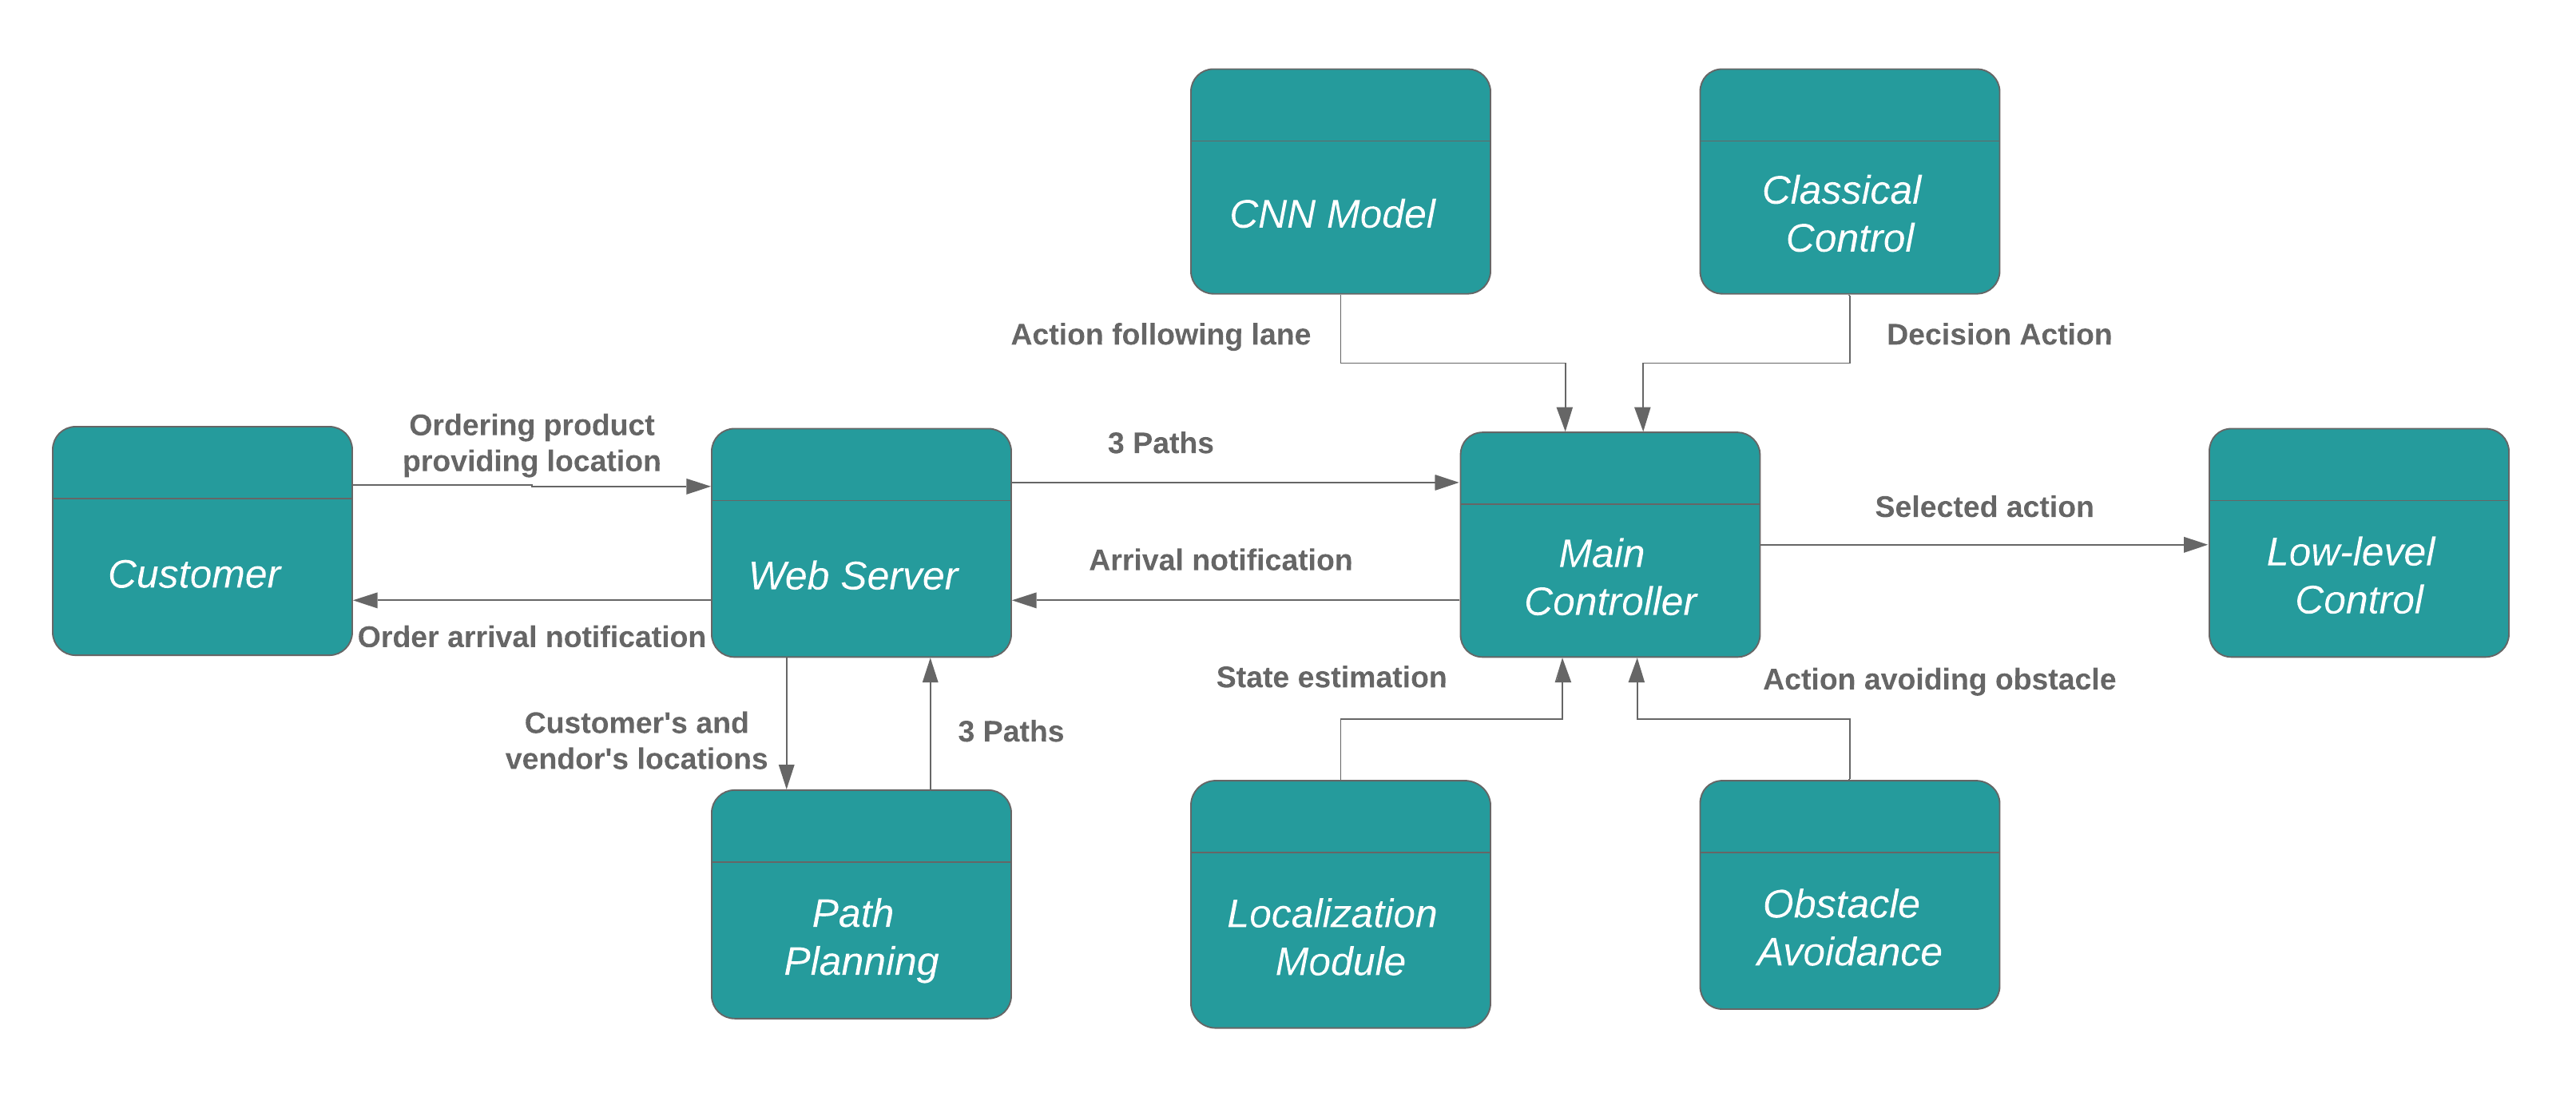
\includegraphics[width=\textwidth]
    {images/Alzahraa/business_scenario.png}%
     % you need to add the caption for the list of figures
    \caption[Business Scenario]{Business scenario}\label{fig:business scenario}%
  \end{figure}

